%\documentclass{beamer} %voce pode usar este modelo tambem
\documentclass[t,handout,9pt]{beamer}
\usepackage{graphicx}
\usepackage{url}
\usepackage[british]{babel}
%\batchmode
% \pgfpagesuselayout{4 on 1}[letterpaper,landscape,border shrink=5mm]
\usepackage{amsmath}
\usepackage{amssymb}
\usepackage{amsfonts}
\usepackage{enumerate}
\usepackage{epsfig}
\usepackage{bbm}
\usepackage{calc}
\usepackage{adjustbox}
\usepackage{color}
\usepackage{ifthen}
\usepackage{capt-of}
\usepackage{float}
\usepackage{booktabs}
\usepackage{dcolumn}
\usepackage{multicol}
\usepackage{hyperref}
\usepackage[flushleft]{threeparttable}
\usepackage{subcaption}
\usepackage{adjustbox}
\usepackage{ragged2e}
\usepackage{pgfpages}
%\usepackage{showframe}

\usepackage{cmbright}

\renewcommand\ttdefault{cmvtt} % selects CM typewriter

\usepackage[utf8]{inputenc} % Required for inputting international characters
\usepackage[T1]{fontenc} 	% Output font encoding for international characters

%\DeclareFontShape{OT1}{cmss}{b}{n}{<->ssub * cmss/bx/n}{}

\usetheme[compress]{Berlin}
\definecolor{sapienza}{RGB}{0, 49, 83}
\usecolortheme[named=sapienza]{structure}

\usepackage[backend=bibtex,style=alphabetic,giveninits=true,url=false,eprint=false,doi=false]{biblatex}
\DeclareNameAlias{sortname}{last-first}
\renewcommand*{\nameyeardelim}{\addcomma\addspace}
\renewcommand*{\bibfont}{\footnotesize}
\addbibresource{example.bib}
\setbeamerfont{footnote}{size=\tiny}

\setbeamerfont{title}{size=\LARGE}

% reduce spaces between tables/figures and caption
\usepackage[font=small,skip=1pt]{caption}

%% pgf plots stuff
%\usepackage{pgfplots}
%\pgfplotsset{compat=newest}
%% the following commands are needed for some matlab2tikz features
%\usetikzlibrary{plotmarks}
%\usetikzlibrary{arrows.meta}
%\usepgfplotslibrary{patchplots}

% one navigation dot per slide trick
\AtBeginSection[]{\subsection{}}

% fix misbehave for allowframebreaks
\usepackage{etoolbox}
\makeatletter
\patchcmd{\slideentry}{\ifnum#2>0}{\ifnum2>0}{}% replace the subsection number test with a test that always returns true
% use frame numbers instead of subsection slide numbers so that frames broken over slides get separate circles
\patchcmd{\slideentry}{\c@subsectionslide}{\c@framenumber}{}{\@error{unable to patch}}
\patchcmd{\beamer@writeslidentry}{\c@subsectionslide}{\c@framenumber}{}{\@error{unable to patch}}

% date in footer trick
\makeatletter
  \setbeamertemplate{footline}{%
    \begin{beamercolorbox}[colsep=1.5pt]{upper separation line foot}
    \end{beamercolorbox}
    \begin{beamercolorbox}[ht=2.5ex,dp=1.125ex,%
      leftskip=.3cm,rightskip=.3cm plus1fil]{author in head/foot}%
      \leavevmode{\usebeamerfont{author in head/foot}\insertshortauthor}%
      \hfill%
      {\usebeamerfont{institute in head/foot}\usebeamercolor[fg]{institute in head/foot}\insertshortinstitute}%
    \end{beamercolorbox}%
    \begin{beamercolorbox}[ht=2.5ex,dp=1.125ex,%
      leftskip=.3cm,rightskip=.3cm plus1fil]{title in head/foot}%
      {\usebeamerfont{title in head/foot}\insertshorttitle\hfill\insertshortdate}%
    \end{beamercolorbox}%
    \begin{beamercolorbox}[colsep=1.5pt]{lower separation line foot}
    \end{beamercolorbox}
  }
\makeatletter

% remove dot for titlepage and Outline
\makeatletter
\let\old@beamer@writeslidentry\beamer@writeslidentry
\def\beamer@writeslidentry{%
  \expandafter\beamer@ifempty\expandafter{\beamer@framestartpage}{}% does not happen normally
  {%else
    \clearpage\beamer@notesactions%
  }
}
\makeatother

% let's number figure captions
\setbeamertemplate{caption}[numbered]

% trick for grouping equations
\newenvironment{rcases}
  {\left.\begin{aligned}}
  {\end{aligned}\right\rbrace}

%-------------------------Titulo/Autores/Orientador------------------------------------------------
\title[Introduction to Computer Programming]{Introduction to Computer Programming}
\date[A.Y. 2024-2025]{\\A.Y. 2024-2025}
\author[Alessio Martino]{Prof. Alessio Martino\\
\smallskip
{\small \href{mailto:amartino@luiss.it}{\texttt{amartino@luiss.it}}}\\
\smallskip
}
\institute[17/09/2024]{Department of Business and Management\\Viale Romania 32, 00197 Rome\\[\bigskipamount]

\includegraphics[scale=0.4]{Figures/cliente-luiss.png}%
}

%-------------------------Logo na parte de baixo do slide------------------------------------------
%\pgfdeclareimage[height=0.7cm]{senac-logo}{senac-logo.pdf}
%\logo{\pgfuseimage{senac-logo}\hspace*{0.5cm}}

%-------------------------Este código faz o menuzinho bacana na parte superior do slide------------
%\AtBeginSection[]
%{
%  \begin{frame}<beamer>
%    \frametitle{Outline}
%    \tableofcontents[currentsection]
%  \end{frame}
%}
%\beamerdefaultoverlayspecification{<+->}
% -----------------------------------------------------------------------------

\begin{document}
% -----------------------------------------------------------------------------

%---Gerador de Sumário---------------------------------------------------------

\frame[noframenumbering]{
	\titlepage
}

% begin personalization stuff
\setbeamertemplate{navigation symbols}{%
	\insertslidenavigationsymbol
	\insertframenavigationsymbol
	\insertsubsectionnavigationsymbol
	\insertsectionnavigationsymbol
	\insertdocnavigationsymbol
	\insertbackfindforwardnavigationsymbol
	\hspace{1em}%
	\usebeamerfont{footline}
	\insertframenumber/\inserttotalframenumber%
}
\setbeamertemplate{itemize items}[circle]
\setbeamertemplate{enumerate items}[circle]
\setbeamertemplate{bibliography item}{\insertbiblabel}
% end personalization stuff

\section[]{}
\begin{frame}{Outline}
	\tableofcontents
\end{frame}
%\begin{frame}{Outline}
%\begin{multicols}{2}
%  \tableofcontents
%\end{multicols}
%\end{frame}
%---Fim do Sumário------------------------------------------------------------

% reset navigation dots for other slides
\makeatletter
\let\beamer@writeslidentry\old@beamer@writeslidentry
\makeatother

% -----------------------------------------------------------------------------
\section{Variables}
\subsection{Variables = a Name for Values}
\begin{frame}{Variables}
The equal sign `\texttt{=}' serves for \textcolor{red}{assigning} a variable name to a value:
\begin{table}[]
\begin{tabular}{ll}
\texttt{>{}>{}> pi = 3.14} & \\
\end{tabular}
\end{table}
where \texttt{pi} is the \textit{variable name} and \texttt{3.14} is the \textit{value}.
\begin{block}{Recall}
The equal sign `\texttt{=}' serves for assignments. The equality check reads as `\texttt{==}'.
\end{block}
Retrieve the value associated to a variable by querying the name on the prompt:
\begin{table}[]
\begin{tabular}{ll}
\texttt{>{}>{}> pi} & $\leftarrow$input  \\
\texttt{3.14}        & $\leftarrow$output
\end{tabular}
\end{table}
\begin{itemize}
	\item All values are stored in the computer memory
	\item The assignment operation binds a name to a value
\end{itemize}
\end{frame}
%
\begin{frame}
Variable names:
\begin{itemize}
	\item must be meaningful
	\item can be as long as you like
	\item can contain both letters and numbers
	\item cannot start with a number
	\item can contain underscores (i.e., `\texttt{\_}')
	\item convention: use only lower letters
	\item Python-reserved keywords are not allowed
\end{itemize}
\begin{table}[]
\centering
\caption{Python 3 Keywords}
\begin{tabular}{lllll}
\texttt{False } & \texttt{class   } & \texttt{finally} & \texttt{is      } & \texttt{return} \\
\texttt{None  } & \texttt{continue} & \texttt{for    } & \texttt{lambda  } & \texttt{try   } \\
\texttt{True  } & \texttt{def     } & \texttt{from   } & \texttt{nonlocal} & \texttt{while } \\
\texttt{and   } & \texttt{del     } & \texttt{global } & \texttt{not     } & \texttt{with  } \\
\texttt{as    } & \texttt{elif    } & \texttt{if     } & \texttt{or      } & \texttt{yield } \\
\texttt{assert} & \texttt{else    } & \texttt{import } & \texttt{pass    } & \texttt{break } \\
\texttt{except} & \texttt{in      } & \texttt{raise  } &          &
\end{tabular}
\end{table}
\end{frame}
%
\begin{frame}
\vfill
Why variable names?
\begin{itemize}
	\item reuse \textcolor{red}{names} instead of \textcolor{red}{values} throughout the code
	\item store (temporarily!) values and results
	\item easier to change the code later
\end{itemize}
\begin{table}[]
\begin{tabular}{ll}
\texttt{>{}>{}> pi=3.14} &  \\
\texttt{>{}>{}> radius=2.2}        & \\
\texttt{>{}>{}> \# calculate the area}        & $\leftarrow$ this is a \textcolor{red}{comment}! \\
\texttt{>{}>{}> area = pi * (radius**2)}        &  \\
\texttt{>{}>{}> \# calculate the diameter}        & \\
\texttt{>{}>{}> diameter = radius*2}        &  \\
\end{tabular}
\end{table}
Syntax of assignments:
\begin{itemize}
	\item rightmost term of assignment: expression that yields a value
	\item leftmost term of assignment: variable name
\end{itemize}
\vfill
\end{frame}
%
\begin{frame}
Variables can be \textcolor{red}{changed} (or \textcolor{red}{re-binded}) using new assignments on the same variable name.
\begin{block}{Warning}
The old value might still be in the computer memory, but you lose the handle for it.
\end{block}
\adjustbox{valign=t}{\begin{minipage}{0.5\textwidth}
\vspace{0.5cm}
\begin{table}[]
\begin{tabular}{ll}
\texttt{>{}>{}> pi=3.14} &  \\
\texttt{>{}>{}> radius=2.2}        & \\
\texttt{>{}>{}> area = pi * (radius**2)}        &  \\
\texttt{>{}>{}> radius = radius+1}        &  \\
\end{tabular}
\end{table}
\begin{block}{Hint}
\texttt{radius = radius+1} can be shortcut to \texttt{radius+=1}.
\end{block}
\begin{block}{Note}
\texttt{area} does not change its value.
\end{block}
\end{minipage}}%
\hfill
\adjustbox{valign=t}{\begin{minipage}[t]{0.49\textwidth}
\vspace{0.3cm}
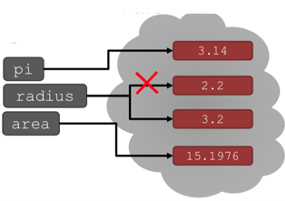
\includegraphics[width=\textwidth]{Figures/Rebinding}
\end{minipage}}
\end{frame}
%
\subsection{Dynamic Typing}
\begin{frame}
Python supports \textcolor{red}{dynamic typing}.
\begin{itemize}
	\item variables can hold values of any type
	\item variables can hold different types throughout the code
\end{itemize}
The following is perfectly valid in Python:
\begin{table}[]
\begin{tabular}{ll}
\texttt{>{}>{}> x=3} &  $\leftarrow$ \texttt{x} now contains an \texttt{int}\\
\texttt{...}        &  \\
\texttt{>{}>{}> x=9.53642}        & $\leftarrow$ \texttt{x} now contains a \texttt{float}  \\
\end{tabular}
\end{table}
\begin{block}{Recall}
You can always use \texttt{type(x)} to find the type of variable \texttt{x}.
\end{block}
You can use \texttt{type()} for comparison and conversion
\begin{table}[]
\begin{tabular}{ll}
\texttt{>{}>{}> x=3} &\\
\texttt{>{}>{}> type(x)==int}        &  \\
\texttt{>{}>{}> x=float(x)}  &  \\
\texttt{>{}>{}> type(x)==float}        &  \\
\end{tabular}
\end{table}
\end{frame}
%------------------------------------------------------------------------------
\section{Strings: a Warmup}
\begin{frame}{Strings: a Warmup}
Strings are objects that can host letters, numbers, spaces, special characters.\\
Strings can be created by enclosing stuff in quotation marks or single quotes:
\begin{table}[]
\begin{tabular}{ll}
\texttt{>{}>{}> hi='hello there'} & $\leftarrow$ or \texttt{"hello there"}\\
\end{tabular}
\end{table}
You can \textcolor{red}{concatenate} strings using the \texttt{+} operator:
\begin{table}[]
\begin{tabular}{ll}
\texttt{>{}>{}> name='alessio'} & \\
\texttt{>{}>{}> greeting=hi + name} & \\
\texttt{>{}>{}> greeting} & \\
\texttt{'hello therealessio'} & \\
\texttt{>{}>{}> greeting=hi + " " + name} & \\
\texttt{>{}>{}> greeting} & \\
\texttt{'hello there alessio'} & \\
\end{tabular}
\end{table}
You can \textcolor{red}{replicate} strings using the \texttt{*} operator:
\begin{table}[]
\begin{tabular}{ll}
\texttt{>{}>{}> name='alessio'} & \\
\texttt{>{}>{}> silly=name*3} & \\
\texttt{>{}>{}> silly} & \\
\texttt{'alessioalessioalessio'} & \\
\end{tabular}
\end{table}
\end{frame}
%
\begin{frame}
\vfill
Single quotes or double quotes can be (in principle) used interchangeably.\\
For example:
\begin{table}[]
\begin{tabular}{ll}
\texttt{>{}>{}> s1 = 'hello students'} & \\
\texttt{>{}>{}> s2 = "hello students"} & \\
\end{tabular}
\end{table}
yield two identical strings.
\vfill
\begin{block}{Problem}
What if my string contains itself a single quote (e.g., \textit{Let's go})?
\end{block}
If we do something like
\begin{table}[]
\begin{tabular}{ll}
\texttt{>{}>{}> s = 'Let's go'} & \\
\end{tabular}
\end{table}
we have an unterminated string syntax error.
\vfill
\begin{block}{Solution}
Wrap your string with single quotes between double quotes!
\end{block}
\vfill
\begin{table}[]
\begin{tabular}{ll}
\texttt{>{}>{}> s = "Let's go"} & \\
\end{tabular}
\end{table}
\vfill
\end{frame}
%
\begin{frame}
\vfill
\begin{block}{(Opposite) problem}
What if my string contains itself a double quote (e.g., \textit{I said "Hello"})?
\end{block}
If we do something like
\begin{table}[]
\begin{tabular}{ll}
\texttt{>{}>{}> s = "I said "Hello""} & \\
\end{tabular}
\end{table}
we have another syntax error, equivalent to the previous one.
\vfill
\begin{block}{Solution}
Wrap your string with double quotes between single quotes!
\end{block}
\vfill
\begin{table}[]
\begin{tabular}{ll}
\texttt{>{}>{}> s = 'I said "Hello"'} & \\
\end{tabular}
\end{table}
\vfill
\end{frame}
%
\begin{frame}
\vfill
\begin{block}{(Yet another) problem}
What if my string contains both single quotes and double quotes (e.g., \textit{I said "What's going on"})?
\end{block}
We cannot do any of the following
\begin{table}[]
\begin{tabular}{ll}
\texttt{>{}>{}> s = "I said "What's going on""} & \\
\texttt{>{}>{}> s = 'I said "What's going on"'} & \\
\end{tabular}
\end{table}
because of syntax errors, equivalent to the previous ones.
\vfill
\begin{block}{Solution}
Wrap your string between triple single quotes!
\end{block}
\vfill
\begin{table}[]
\begin{tabular}{ll}
\texttt{>{}>{}> s = '''I said "What's going on"'''} & \\
\end{tabular}
\end{table}
\vfill
\end{frame}
%
\subsection{Escape Sequences}
\begin{frame}
\vfill
We can solve the above problem also thanks to \textcolor{red}{escape sequences}.
\vfill
Escape sequences are brief sequences of characters that start with a backslash and are interpreted differently.
\vfill
There exist escape sequences to display single quotes (\texttt{\textbackslash'}) and double quotes (\texttt{\textbackslash"}) ... and to display the backslash itself (\texttt{\textbackslash\textbackslash}):
\begin{itemize}
	\item if we 'shield' single or double quotes with a backslash, they are interpreted as characters rather than string delimiters;
	\item if we 'shield' the backslash with a backslash, it is interpreted as character rather than 'this the beginning of an escape sequence'.
\end{itemize}
\vfill
Let's try the following:
\begin{table}[]
\begin{tabular}{ll}
\texttt{>{}>{}> s1 = 'I said "What\textbackslash's going on"'} & \\
\texttt{>{}>{}> s2 = "I said \textbackslash"What's going on\textbackslash""} & \\
\texttt{>{}>{}> s3 = "Hello\textbackslash\textbackslash Students"} & \\
\end{tabular}
\end{table}
\vfill
\end{frame}
%
\begin{frame}
\vfill
There exist escape sequences also for string formatting.
\vfill
Let's see the most important ones:
\begin{itemize}
	\item new line \texttt{\textbackslash n}, which changes the line and takes the cursor to the beginning of a new line
	\item tab space \texttt{\textbackslash t}, which leaves a horizontal tab space
	\item carriage return \texttt{\textbackslash r}, which moves the cursor back to the beginning of the line
	\item alarm \texttt{\textbackslash a}, which plays the system alarm (bell)
	\item form feed \texttt{\textbackslash v} or \texttt{\textbackslash f}, which breaks the line
\end{itemize}
\vfill
Let's see them in action:
\begin{table}[]
\begin{tabular}{ll}
\texttt{>{}>{}> s1 = 'Hello\textbackslash nStudents'} & \\
\texttt{>{}>{}> s2 = 'Hello\textbackslash tStudents'} & \\
\texttt{>{}>{}> s3 = 'Hello\textbackslash rStudents'} & \\
\texttt{>{}>{}> s4 = 'Hello\textbackslash vStudents'} & \\
\texttt{>{}>{}> print('\textbackslash a')} & \\
\end{tabular}
\end{table}
\vfill
\end{frame}
%------------------------------------------------------------------------------
\section{Input/Output}
\subsection{Output: \texttt{print()}}
\begin{frame}{Input/Output}
\begin{itemize}
	\item Show some stuff to the command line
	\item Universal (and very flexible) keyword: \texttt{print()}
\end{itemize}
Examples:
\begin{table}[]
\begin{tabular}{ll}
\texttt{>{}>{}> print('apple', 'banana')} & $\leftarrow$ two input arguments\\
\texttt{'apple banana'} & \\
\texttt{>{}>{}> print('apple' + 'banana')} & $\leftarrow$ one input arguments\\
\texttt{'applebanana'} & \\
\end{tabular}
\end{table}
By default, multiple input arguments are separated by space ('\texttt{ }') and the line terminates with a newline ('\texttt{$\backslash$n}'). You can change that via \texttt{sep} and \texttt{end}.\\
Example:
\begin{table}[]
\begin{tabular}{ll}
\texttt{>{}>{}> a=5} & \\
\texttt{>{}>{}> print("a=", a, 10, "bye", sep='|', end='$\backslash$n$\backslash$n$\backslash$n')} & \\
\texttt{a=|5|10|bye} & \\
\texttt{} & $\leftarrow$ blank line\\
\texttt{} & $\leftarrow$ blank line\\
\texttt{>{}>{}>} & \\
\end{tabular}
\end{table}
\end{frame}
%
\begin{frame}
\vfill
Hence, there are two strategies to print something on screen:
\begin{enumerate}
	\item pass multiple arguments to \texttt{print()} and it automatically takes care of printing strings, numbers and different data types
	\item build your own string and just \texttt{print()} it.
\end{enumerate}
\vfill
The second case deserves further observations.
\vfill
What happens if we run the following code?
\begin{table}[]
\begin{tabular}{ll}
\texttt{>{}>{}> age=5} & \\
\texttt{>{}>{}> name='Eric'} & \\
\texttt{>{}>{}> print("My name is "+name+" and I'm "+age+" years old.")} & \\
\end{tabular}
\end{table}
It will error because we cannot concatenate (i.e., \texttt{+}) strings and numbers together.\\
Hence, we must convert \texttt{myage} to string (i.e., using \texttt{str()}).
\vfill
\end{frame}
%
\subsection{String Formatting}
\begin{frame}
\vfill
Luckily, Python has several string formatting shortcuts that allow us to create strings
\begin{itemize}
	\item without manual concatenation and casting
	\item in a very elegant and clean way.
\end{itemize}
\vfill
Let's see the old-school way (C-like).
\vfill
What happens if we run the following code?
\begin{table}[]
\begin{tabular}{ll}
\texttt{>{}>{}> n1 = 5} & \\
\texttt{>{}>{}> n2 = 1234.56789} & \\
\texttt{>{}>{}> print("The value of n1 is \%d" \%n1)} & \\
\texttt{>{}>{}> print("The value of n2 is \%d" \%n2)} & \\
\texttt{>{}>{}> print("The value of n1 is \%f" \%n1)} & \\
\texttt{>{}>{}> print("The value of n2 is \%f" \%n2)} & \\
\end{tabular}
\end{table}
\vfill
\end{frame}
%
\begin{frame}
\vfill
In the string we are building, we can see that:
\begin{itemize}
	\item the percentage sign marks the place where the value has to be inserted
	\item \texttt{\%} is followed by the conversion format, i.e.:
	\begin{itemize}
		\item \texttt{\%d} stands for decimal (i.e., integer)
		\item \texttt{\%f} stands for floating point
	\end{itemize}
	\item the format automatically performs casting
	\begin{itemize}
		\item \texttt{n1} is an integer, but it renders as float if we use \texttt{\%f}
		\item \texttt{n2} is a float, but it renders as integer if we use \texttt{\%d}
	\end{itemize}
\end{itemize}
\vfill
Outside the string we are building, we note that:
\begin{itemize}
	\item \texttt{\%} is followed by the variable name (or value) we want to plug inside the string
\end{itemize}
\vfill
\begin{block}{Note}
We can personalize \texttt{\%f} by specifying the number of digits before and after the decimal separator. That is, \texttt{\%$x$.$y$f} yields a floating point number with \texttt{$x$} digits before and \texttt{$y$} digits after the comma. \texttt{$x$} can be omitted.
\end{block}
\vfill
\end{frame}
%
\begin{frame}
\vfill
We can build strings with an arbitrary number of placeholders.
\vfill
Let's run the following code
\begin{table}[]
\begin{tabular}{ll}
\texttt{>{}>{}> name = "Eric"} & \\
\texttt{>{}>{}> age = 5} & \\
\texttt{>{}>{}> print("My name is \%s and I'm \%d years old." \%(name, age))} & \\
\end{tabular}
\end{table}
\vfill
We note that:
\begin{itemize}
	\item we have two placeholders inside the string
	\begin{itemize}
		\item \texttt{\%s} stands for strings
		\item \texttt{\%d} follows from previous slide
	\end{itemize}
	\item outside the string, we have our variables/values collected in round brackets\footnote{That's a \textit{tuple}, we will see tuples later in the course.}
	\item the order of the placeholders must match the ones in the tuple
\end{itemize}
\vfill
\begin{block}{Note}
\texttt{\%s} can be used for strings and for all objects that support a string conversion, e.g., numbers.
\end{block}
\vfill
\end{frame}
%
\subsection{Input: \texttt{input()}}
\begin{frame}{Input/Output}
\vfill
\begin{itemize}
	\item Ask the user for some input via keyboard
	\item Keyword: \texttt{input('...')}
\end{itemize}
\vfill
How does it work?:
\begin{enumerate}
	\item prints whatever is in the quotes
	\item user types something and press Enter
	\item binds the value to a variable
\end{enumerate}
\vfill
Example:
\begin{table}[]
\begin{tabular}{ll}
\texttt{>{}>{}> text=input('Type something: ')} & \\
\texttt{Type something: hello} & $\leftarrow$ \texttt{hello} is written by the user\\
\texttt{>{}>{}> print(text*3)} & \\
\texttt{'hellohellohello'} & \\
\end{tabular}
\end{table}
\vfill
\end{frame}
%
\begin{frame}
\vfill
\begin{block}{Warning}
\texttt{input()} always returns a string. If you have to play with numbers, you must cast.
\end{block}
\vfill
Example:
\begin{table}[]
\begin{tabular}{ll}
\texttt{>{}>{}> num=input('Enter a number: ')} & \\
\texttt{Enter a number: 5} & $\leftarrow$ \texttt{5} is written by the user\\
\texttt{>{}>{}> num} & \\
\texttt{'5'} & \\
\texttt{>{}>{}> type(num)} & \\
\texttt{'str'} & \\
\texttt{>{}>{}> num = int(num)} & \\
\texttt{>{}>{}> type(num)} & \\
\texttt{int} & \\
\end{tabular}
\end{table}
\vfill
\end{frame}
%------------------------------------------------------------------------------
\section{Some Recaps}
\subsection{Data Types}
\begin{frame}{Some Recaps}
\begin{itemize}
	\item Type: \texttt{int}
	\begin{itemize}
		\item values: integers
		\item operations: \texttt{+}, \texttt{-}, \texttt{/}, \texttt{//}, \texttt{*}, \texttt{\%}, \texttt{**}, ...
	\end{itemize}
	\item Type: \texttt{float}
	\begin{itemize}
		\item values: real numbers
		\item operations: \texttt{+}, \texttt{-}, \texttt{/}, \texttt{//}, \texttt{*}, \texttt{\%}, \texttt{**}, ...
	\end{itemize}
	\item Type: \texttt{bool}
	\begin{itemize}
		\item values: \texttt{True} and \texttt{False}
		\item operations: \texttt{or}, \texttt{and}, \texttt{not}
	\end{itemize}
	\item Type: \texttt{str}
	\begin{itemize}
		\item values: string literals
		\item operations: \texttt{+}, \texttt{*}, ...
	\end{itemize}
\end{itemize}
\begin{block}{Note}
We will see more (non-scalar) data types later in the course.
\end{block}
\end{frame}
%
\subsection{Interactive vs. Script}
\begin{frame}
\vfill
What happens if you type this code in the interpreter or write a script and execute it?\\
\begin{table}[]
\begin{tabular}{ll}
\texttt{>{}>{}> miles = 11.41} & \\
\texttt{>{}>{}> miles} & \\
\texttt{>{}>{}> miles * 2} & \\
\end{tabular}
\end{table}
\begin{table}[]
\begin{tabular}{@{}cc@{}}
\toprule
\textbf{Interactive}                  & \textbf{Script}          \\ \midrule
Assignments are silent                & Assignments are silent   \\
Variable query returns its content    & Variable query is silent \\
Expressions are returned in real-time & Expressions are silent   \\ \bottomrule
\end{tabular}
\end{table}
\begin{block}{Note}
If you want your script to show something, you must use \texttt{print()}.
\end{block}
\vfill
\end{frame}
%
\subsection{Expressions vs. Statements}
\begin{frame}
\vfill
So, we can say that:
\begin{description}
\item[Expressions:] \textcolor{red}{Represent} something\\
\begin{itemize}
	\item Python \textit{evaluates} expressions
	\item end-result is a value
\end{itemize}
Examples:
\begin{table}[]
\begin{flushleft}
\begin{tabular}{ll}
\texttt{>{}>{}> 2.3} & $\leftarrow$ a plain literal\\
\texttt{>{}>{}> (7*3+1)-4} & $\leftarrow$ 4 literals and some operators\\
\end{tabular}
\end{flushleft}
\end{table}
\item[Statements:] \textcolor{red}{Do} something\\
\begin{itemize}
	\item Python \textit{executes} statements
	\item no need to return a value
\end{itemize}
Examples:
\begin{table}[]
\begin{flushleft}
\begin{tabular}{ll}
\texttt{>{}>{}> print("Hi there!")} & \\
\texttt{>{}>{}> import sys} & \\
\end{tabular}
\end{flushleft}
\end{table}
\end{description}
\vfill
\end{frame}
%------------------------------------------------------------------------------
%\section{Input/Output}
%\subsection{Output: \texttt{print()}}
%\begin{frame}{Input/Output}
%\begin{itemize}
%	\item Show some stuff to the command line
%	\item Universal (and very flexible) keyword: \texttt{print()}
%\end{itemize}
%Examples:
%\begin{table}[]
%\begin{tabular}{ll}
%\texttt{>{}>{}> print('apple', 'banana')} & $\leftarrow$ two input arguments\\
%\texttt{'apple banana'} & \\
%\texttt{>{}>{}> print('apple' + 'banana')} & $\leftarrow$ one input arguments\\
%\texttt{'applebanana'} & \\
%\end{tabular}
%\end{table}
%By default, multiple input arguments are separated by space ('\texttt{ }') and the line terminates with a newline ('\texttt{$\backslash$n}'). You can change that via \texttt{sep} and \texttt{end}.\\
%Example:
%\begin{table}[]
%\begin{tabular}{ll}
%\texttt{>{}>{}> a=5} & \\
%\texttt{>{}>{}> print("a=", a, 10, "bye", sep='|', end='$\backslash$n$\backslash$n$\backslash$n')} & \\
%\texttt{a=|5|10|bye} & \\
%\texttt{} & $\leftarrow$ blank line\\
%\texttt{} & $\leftarrow$ blank line\\
%\texttt{>{}>{}>} & \\
%\end{tabular}
%\end{table}
%\end{frame}
%%
%\subsection{Input: \texttt{input()}}
%\begin{frame}{Input/Output}
%\vfill
%\begin{itemize}
%	\item Ask the user for some input via keyboard
%	\item Keyword: \texttt{input('...')}
%\end{itemize}
%\vfill
%How does it work?:
%\begin{enumerate}
%	\item prints whatever is in the quotes
%	\item user types something and press Enter
%	\item binds the value to a variable
%\end{enumerate}
%\vfill
%Example:
%\begin{table}[]
%\begin{tabular}{ll}
%\texttt{>{}>{}> text=input('Type something: ')} & \\
%\texttt{Type something: hello} & $\leftarrow$ \texttt{hello} is written by the user\\
%\texttt{>{}>{}> print(text*3)} & \\
%\texttt{'hellohellohello'} & \\
%\end{tabular}
%\end{table}
%\vfill
%\end{frame}
%%
%\begin{frame}
%\vfill
%\begin{block}{Warning}
%\texttt{input()} always returns a string. If you have to play with numbers, you must cast.
%\end{block}
%\vfill
%Example:
%\begin{table}[]
%\begin{tabular}{ll}
%\texttt{>{}>{}> num=input('Enter a number: ')} & \\
%\texttt{Enter a number: 5} & $\leftarrow$ \texttt{5} is written by the user\\
%\texttt{>{}>{}> num} & \\
%\texttt{'5'} & \\
%\texttt{>{}>{}> type(num)} & \\
%\texttt{'str'} & \\
%\texttt{>{}>{}> num = int(num)} & \\
%\texttt{>{}>{}> type(num)} & \\
%\texttt{int} & \\
%\end{tabular}
%\end{table}
%\vfill
%\end{frame}
%%
%\section{Types (Recap)}
%\begin{frame}{Types (Recap)}
%\begin{itemize}
%	\item Type: \texttt{int}
%	\begin{itemize}
%		\item values: integers
%		\item operations: \texttt{+}, \texttt{-}, \texttt{/}, \texttt{//}, \texttt{*}, \texttt{\%}, \texttt{**}, ...
%	\end{itemize}
%	\item Type: \texttt{float}
%	\begin{itemize}
%		\item values: real numbers
%		\item operations: \texttt{+}, \texttt{-}, \texttt{/}, \texttt{//}, \texttt{*}, \texttt{\%}, \texttt{**}, ...
%	\end{itemize}
%	\item Type: \texttt{bool}
%	\begin{itemize}
%		\item values: \texttt{True} and \texttt{False}
%		\item operations: \texttt{or}, \texttt{and}, \texttt{not}
%	\end{itemize}
%	\item Type: \texttt{str}
%	\begin{itemize}
%		\item values: string literals
%		\item operations: \texttt{+}, \texttt{*}, ...
%	\end{itemize}
%\end{itemize}
%\begin{block}{Note}
%We will see more data types later in the course.
%\end{block}
%\end{frame}
%%
%\section{Interactive vs. Script}
%\begin{frame}{Interactive vs. Script}
%What happens if you type this code in the interpreter or write a script and execute it?\\
%\begin{table}[]
%\begin{tabular}{ll}
%\texttt{>{}>{}> miles = 11.41} & \\
%\texttt{>{}>{}> miles} & \\
%\texttt{>{}>{}> miles * 2} & \\
%\end{tabular}
%\end{table}
%\begin{table}[]
%\begin{tabular}{@{}cc@{}}
%\toprule
%\textbf{Interactive}                  & \textbf{Script}          \\ \midrule
%Assignments are silent                & Assignments are silent   \\
%Variable query returns its content    & Variable query is silent \\
%Expressions are returned in real-time & Expressions are silent   \\ \bottomrule
%\end{tabular}
%\end{table}
%\begin{block}{Note}
%If you want your script to show something, you must use \texttt{print()}.
%\end{block}
%\end{frame}
%%
%\section{Expressions vs. Statements (Recap)}
%\begin{frame}{Expressions vs. Statements (Recap)}
%So, we can say that:
%\begin{description}
%	\item[Expressions:] \textcolor{red}{Represent} something\\
%	\begin{itemize}
%		\item Python \textit{evaluates} expressions
%		\item end-result is a value
%	\end{itemize}
%	Examples:
%	\begin{table}[]
%	\begin{flushleft}
%	\begin{tabular}{ll}
%	\texttt{>{}>{}> 2.3} & $\leftarrow$ a plain literal\\
%	\texttt{>{}>{}> (7*3+1)-4} & $\leftarrow$ 4 literals and some operators\\
%	\end{tabular}
%	\end{flushleft}
%	\end{table}
%	\item[Statements:] \textcolor{red}{Do} something\\
%	\begin{itemize}
%		\item Python \textit{executes} statements
%		\item no need to return a value
%	\end{itemize}
%	Examples:
%	\begin{table}[]
%	\begin{flushleft}
%	\begin{tabular}{ll}
%	\texttt{>{}>{}> print("Hi there!")} & \\
%	\texttt{>{}>{}> import sys} & \\
%	\end{tabular}
%	\end{flushleft}
%	\end{table}
%\end{description}
%\end{frame}
%------------------------------------------------------------------------------
%\section{References}
%\begin{frame}[allowframebreaks]{References}
%%\bibliographystyle{apacite}
%\printbibliography[heading=none]
%\end{frame}
\section{References}
\begin{frame}{References}
	Variables and Strings:
\begin{itemize}
	\item Guttag, J. V. (2013). \textit{Introduction to Computation and Programming using Python (Revised and Expanded Edition)}. MIT Press. [Section 2.1.2 and 2.3]
	\item Downey, A. (2015). \textit{Think Python}. Green Tea Press ed. 2nd. [Sections 2.1--2.2, 2.6--2.7]
\end{itemize}
Input/Output:
\begin{itemize}
	\item Guttag, J. V. (2013). \textit{Introduction to Computation and Programming using Python (Revised and Expanded Edition)}. MIT Press. [Chapter 2]
	\item Downey, A. (2015). \textit{Think Python}. Green Tea Press ed. 2nd. [Sections 2.3--2.4, 5.11]
	\item \url{https://realpython.com/python-print/}
\end{itemize}
\end{frame}
%------------------------------------------------------------------------------
\section{Acknowledgments}
\begin{frame}{Acknowledgments}
%\begin{itemize}
%	\item Prof. Irene Finocchi (LUISS University)\\
%	\quad \textit{Introduction to Computer Programming} Lecture Notes (2020-2021)
%\end{itemize}
\end{frame}
%------------------------------------------------------------------------------
%\subsection{Sites legais}
%\begin{frame}{Sites legais}
%  Want to know more? See!
%  \begin{itemize}
%    \item Browse in my page \url{http://www.ezefranca.com}.
%    \item Browse on BCC page \url{http://www.sp.senac.br/bcc}.
%    \item Thanks WriteLaTeX from Support! \url{http://www.writelatex.com}.
%  \end{itemize}
%
%\end{frame}
%------------------------------------------------------------------------------

% -----------------------------------------------------------------------------
\end{document}
%-----------------------------------------------Este comentario nunca aparecera
